%From introduction to be added here

%Data transfer and storage are expensive for research data centers as well as Internet-of-Things (IoT) devices\footnote{Dataversity, \href{https://www.dataversity.net/internet-things-vs-edge-computing-processing-real-time-data/}{Internet of Things vs. Edge Computing: Processing Real-Time Data}, accessed online 12/2018}.

%(including inter/multidisciplinary, intersectoral and, where appropriate, gender aspects)

\subsubsection{Introduction, objectives and overview of the research program}
\label{sec:introRO}

%\noindent{\color{blue}{State of the art and how \acronym will go beyond it}.}
%brief description, international bibliographic references, cite the consortium

Researchers in HEP study the basic constituents of matter and their interactions within the theory called the Standard Model (SM), and search for new physics phenomena explaining the SM's shortcomings. 
One of the main experimental tools available for this study is the LHC. 
At the LHC, particle beams are accelerated to high energies and 
collision \textit{events} occur 30 million times per second. 
The products of the collisions are analyzed by scientists operating four main particle detectors: ALICE, ATLAS, CMS and LHCb\footnote{CERN, \href{http://cds.cern.ch/record/1997374}{The LHC Experiments}, CERN Document Server}.
Recording each event would require 1000 times the available storage, and in many cases over 10 times the available data acquisition bandwidth.
Each experiment therefore has a \textit{trigger system} composed of hardware and software.
The trigger system analyzes collision events in real time, with a maximum delay of micro- to milliseconds, and selects the ones most interesting for further analysis. 
While there are many observed phenomena that are still not included in the SM (e.g. dark matter~\footnote{Doglioni and Boveia, \href{https://arxiv.org/abs/arXiv:1810.12238}{Dark Matter searches at colliders}, Ann.Rev.Nucl.Part.Sci. 68 (2018) 429-459}), the leading predictive theories such as Supersymmetry have not yet yielded a discovery. 
This is prompting HEP researchers to reconsider their definition of "interesting". 
New phenomena could have unexpected, not-yet-theorized manifestations in the detector, and they would be missed using the current trigger algorithms. 
New phenomena could also be extremely rare and buried in uninteresting backgrounds, and require specialized data taking techniques. 
Moreover, disagreements of data with the SM prediction require dedicated investigation with the new dataset, and therefore dedicated trigger reconstruction and selection criteria. 
For example, the SM prediction that the weak force couples equally to all lepton types (Lepton Flavor Universality, or LFU) has recently been challenged by LHCb measurements~\footnote{LHCb Collaboration, \href{https://arxiv.org/abs/1705.05802}{Test of lepton universality with $ B^{+}\rightarrow K^{+}\ell^{+}\ell$}, Phys. Rev. Lett. 113, 151601 (2014). LHCb Collaboration, \href{https://arxiv.org/abs/1705.05802}{Test of lepton universality with $B^{0}\rightarrow K^{* 0}\ell^{+}\ell$}, JHEP 08 (2017) 055.}. This makes LFU and LFV (Lepton Flavor Violation, the prediction that the overall number of leptons of a given type does not change in interactions) among the most interesting topics for the near-future of particle physics. 
Measurements of LFU and LFV are only one of the many examples that need RTA to be explored in detail with the upcoming LHC dataset. 
\acronym will train a new generation of researchers with a strong expertise on RTA techniques and analysis of large datasets. 
The ESRs will \textbf{exploit innovative ML techniques and hybrid computing architectures to upgrade the trigger systems of LHC experiments for the next LHC data taking periods where the volume of data will increase tenfold}. 
The ESR in \acronym will deploy the necessary RTA tools and use them to \textbf{perform measurements to verify the SM to a high precision and to search for new, unexpected physics phenomena that can shed light on the open questions of the fundamental components of matter}. 

As detailed in Secs.~\ref{sec:trainingcontrib} and~\ref{ss:competence_44}, researchers in the \acronym consortium are experts on the trigger systems of all four main LHC experiments. 
Within \acronym, they will pool their expertise and complement it with that of computer scientists, entrepreneurs and professionals. 
With this consortium, \acronym can \textbf{strengthen European innovation capacity, recognizing that RTA methods solve both academic research and industry challenges}, can be transferred from research to industry and vice versa leading to concrete deliverables.

\acronym's ESR projects employ RTA in projects that are useful to industry and society. 
Time-to-insight from raw data is a crucial benchmark for a competitive and effective use of the information. For this reason, advancement in terms of fast and efficient data analysis and decision-making are required by society and the commercial sector, and a selection of example industrial use cases sharing common issues with HEP has been chosen as integral part of the \acronym research and exploitation program as described further in Sec.~\ref{sec:exploit}.  
RTA is a key point for improving transport and its safety, as well as for optimizing industrial processes. 
The information on the position of private or public transport vehicles and their possible routes are transmitted to a central analysis system, so that the traffic conditions around it are analyzed and a forecast is made. 
All of this needs to be done on a timescale that is short enough for a city to modify its traffic light system to avoid congestion, or to reroute vehicles to avoid delays. 
This requires both ML and hybrid computing architectures for algorithm training, similarly to the solution of complex problems such as tracking particles in a HEP detector. 
The detection of a driver's behavior (e.g. drowsiness) in fleets of cars needs to happen in the timescale of milliseconds to preserve safety, and detection of malfunctioning components in industrial processes must trigger maintenance before the component breaks. Both those use cases require the optimization of advanced algorithms on limited computational resources, much like HEP's trigger systems.
Another use case for RTA in industry is fraud detection, where spotting an anomalous transaction and deciding whether it is allowed or not needs to be made on a short timescale. This is a similar challenge to HEP triggers looking for unexpected phenomena. 
While ML algorithms trained to detect outliers are the current state of the art for this purpose, their black box approach raises interpretability and explainability challenges. 
This is one of the topics beyond the state-of-the-art that is tackled by \acronym: knowledge-based approaches for the induction of explicit decision rules are useful both for increasing the accountability of fraud detection algorithms and for HEP trigger systems where every decision to discard an event is final and must be completely understood.\\
%\vskip-10pt
%\noindent
\fbox{\begin{minipage}{0.985\textwidth}
\textbf{In summary, \acronym trains researchers in ML, AI and data analysis and hybrid computing architectures, so they can enable RTA for the advancement of decision-making as well as monitoring and discoveries in both research and industry. 
The work and expertise developed within \acronym will develop and commission upgraded trigger systems for LHC experiments for HEP measurements and searches, improve transport~\footnote{According to the \href{https://ec.europa.eu/programmes/horizon2020/en/h2020-section/smart-green-and-integrated-transport}{H2020 Societal Challenge for Smart, green and integrated transport}}, industrial process and financial decision-making.}
\end{minipage}}

%\fbox{\begin{minipage}{0.985\textwidth}
%\textbf{Within \acronym, the cross-pollination on RTA between academia and example use cases in industry will lead to concrete deliverables with a focus on 
%enhancing the capabilities and reproducibility of decision-making in finance,
%improving industrial processes, and on
%improving European transport ).
%}
%\end{minipage}}

\subsubsection*{Consortium composition}

\acronym spans ten different countries. 
\cernentity, the \nikhefentity and \cnrsentity research organizations, and universities \sorbonneentity, \helsinkientity, \unigeentity, \dortmundentity, \lundentity, \heidelbergentity form the core academic side of the Network, with experts in HEP and computer science.
\ibmentity and \fleetmaticsentity as beneficiaries, and \ximantisentity, \lightboxentity, \pointeightentity, as partners, form a balanced counterpart to academia with a focus on the same technological challenges as HEP to gain insight into data in real-time. 
\oregonentity, \ohioentity, \pisaentity, \santiagoentity, \liegesentity, \radboudentity and \amsterdamentity are high-profile associated academic partners whose expertise reinforces the network, that provide training and secondment to the ESRs, and award PhD degrees in case the beneficiaries are industries and research institutes\footnote{In this proposal, we use "node" to indicate
either beneficiary or partner. The \textit{node responsible} is the \textit{main scientific contact person} for the node. Administrators, albeit indispensable for the network functioning, are not named even if they are node responsibles in the case scientists are affiliated to two nodes.}.
All consortium members have successfully proven their capabilities for research, training, exploitation and dissemination as shown in Sec.~\ref{sec:supervision},~\ref{ss:competence_44} and part B2.

\subsubsection*{Network goals and research objectives}

As introduced in Sec.~\ref{sec:introRO}, the \acronym ESRs will be trained in:
\begin{itemize}
\item ML techniques and advanced data analysis;
\item hybrid computing architectures;
\item real-time decision making;
\item real-time monitoring of complex processes and discovery of unexpected phenomena.
\end{itemize}

These training goals define the four main research topics for \acronym, each corresponding to a research Work Package (WP) detailed in Sec.~\ref{sec:metho}, with objectives and outcomes shown in each table in this Section that can be reached thanks to collaboration between industry and HEP.  
The first two topics, ML and hybrid architectures, provide the research tools so that RTA methods can used for the latter two topics, with concrete deliverables in physics and industry listed in Sec.~\ref{sub:WPsDescription}.  

%\vspace{-2mm}
%\begin{multicols}{2}[]
%%\footnotesize
%\begin{enumerate}%{\leftmargin=1em}

The first research topic concerns the use of \textbf{ML and advanced data analysis} in RTA techniques.
%The sheer size of the datasets collected by scientific experiments has lead researchers in HEP to use advanced data analysis methods normally used in industry, such as ML and AI. 
ML techniques are by now ubiquitous in both HEP and industry, in order to optimally analyze raw, unstructured data. 
In \acronym we will further extend their use in RTA and event reconstruction, paying particular attention to their understandability and reproducibility (see research topic 4).
Meta-analysis (benchmarking) is also necessary to understand the algorithm performance prior to using them in RTA and to satisfy he requirements of resource-constrained environments.

\begin{center}
\vskip-15pt
\resizebox {\textwidth }{!}{%
\footnotesize
\begin{tabular}{|p{0.5\textwidth}|p{0.5\textwidth}|}
%\toprule
\hline
\textbf{Research Objective:} & \textbf{Outcomes:} \\
\hline
design and use a variety of ML algorithms for RTA (GAN, RNN, Deep Learning)  & toolkits to be used in HEP and commercially;\\
\hline
implement efficient real-time object and event reconstruction & software for HEP experiment triggers;\\
\hline
benchmark and optimize RTA algorithm performance & inter-sector benchmarking toolkits;\\
\hline
%\bottomrule
%\vspace{-1cm}
\end{tabular}
}
\end{center}
%\end{table}
%\vskip5pt

The second research topic focuses on the design of innovative \textbf{hybrid computing architecture} solutions in hardware/software, given that the complexity and rate of LHC data and beyond does not allow standard processors or data analysis techniques to be competitive\footnote{J.P. Vlimant, \href{https://erez.weizmann.ac.il/pls/htmldb/f?p=101:58:::NO:RP:P58_CODE,P58_FILE:5393,Y}{Machine Learning in Charged Particle Tracking}, Hammers and Nails ML\&HEP Conference, 2017}. An example of such a technology in HEP is the Fast TracKer in ATLAS, a hardware-based ATLAS Fast TracKer (FTK)\footnote{J Adelman et al., \href{https://inspirehep.net/record/1614024/}{ATLAS FTK Challenge: Simulation of a Billion-fold Hardware Parallelism,} Procedia Comput.Sci. 66 (2015) 540-545}, a unique hardware processor made by several custom electronic boards based on Field Programmable Gate Arrays (FPGA) to reconstruct the trajectory (track) of the charged particles that cross the inner part of the experiment. In industry, Graphic Processing Units (GPU) are used for computing parallel processes and training ML algorithms, and their use is being prototyped in HEP by members of \acronym. 
\begin{center}
\vskip-15pt
\resizebox {\textwidth }{!}{%
\footnotesize
\begin{tabular}{|p{0.5\textwidth}|p{0.5\textwidth}|}
%\toprule
\hline
\textbf{Research Objective:} & \textbf{Outcomes:} \\
\hline
use of FPGAs for fast hardware computations & trigger improvements for LHC experiments;\\
\hline
use of GPUs for massively parallel computations & significant speed-up for HEP and industrial ML and RTA techniques;\\
\hline
design parallelized and multithreaded algorithms & RTA software needed for the increase in LHC data and for more efficient financial transactions;\\
\hline
%\bottomrule
%\vspace{-1cm}
\end{tabular}
}
\end{center}
%\end{table}
%\vskip5pt

The third research topic concerns \textbf{real-time decision making in physics and industry}. 
The outcomes of the previous research topics will be applied to concrete physics cases and industrial challenges. 
These improvements in RTA benefit each experiment's physics program and increase the information quality extracted from data-rich environments in industry.  
There are many HEP drivers behind the trigger improvements that will be the \acronym ESR's thesis topics: hints of physics beyond the SM in LFV/LFU, the mystery of 85\% of the matter content of the universe that is not yet included in the SM, the in-depth study of the newly discovered Higgs boson and the study of collective particle behavior from states of matter created shortly after the Big Bang. Similar techniques used for trigger improvements will also help improve transport and fleet safety. 
\begin{center}
\vskip-15pt
\resizebox {\textwidth }{!}{%
\footnotesize
\begin{tabular}{|p{0.5\textwidth}|p{0.5\textwidth}|}
%\toprule
\hline
\textbf{Research Objective:} & \textbf{Outcomes:} \\
\hline
deploy improvements from real-time reconstruction and hybrid architectures in HEP trigger systems & measurements and searches with LHC Run-3 data;\\
\hline
use ML and hybrid architecture for RTA to improve transport and safety of fleets & inputs to traffic management of connected cities, extended transport apps and in-vehicle software;\\
\hline
%\bottomrule
%\vspace{-1cm}
\end{tabular}
}
\end{center}
%\end{table}
%\vskip5pt

The fourth research topic concerns efficient and accountable \textbf{monitoring} of complex processes and increase the sensitivity to physics \textbf{discoveries} through outlier detection and novel RTA techniques in data taking. 

Firstly, industry and HEP share the challenge of not knowing in advance what kind of "interesting" events will appear, in the case of malfunctioning equipment, fraudulent financial transaction or potential not-yet-theorised new physics process. 
Outlier/novelty detection is a growing field, with dedicated ML algorithms\footnote{R. Domingues et al, \href{A comparative evaluation of outlier detection algorithms: experiments and analyses}{http://doi.org/10.1016/j.patcog.2017.09.037}, Pattern Recognition 74 (2018)}. In \acronym, experts in the field and their supervised ESRs will apply those to physics and industry use cases, and extending them to methods where rules on what are inferred from a mixture of theory and known events to increase their accountability and understandability.

Secondly, the present HEP paradigm is to select in real-time a small number of interesting events, but keep the full detector data for later analysis. This paradigm depends on the assumption that interesting events are very rare compared to the SM backgrounds. It is however becoming increasingly clear that crucial HEP research questions can only be answered by either precise measurements of the abundant SM processes themselves, or by searching for new processes which closely mimic these SM backgrounds~\footnote{See e.g. Gligorov and Fitzpatrick, \href{http://cds.cern.ch/record/1670985}{Anatomy of an upgrade event in the upgrade era, and implications for the LHCb trigger}, CDS Document Server and ALICE Collaboration including Christiansen, \href{https://cds.cern.ch/record/2011297/files/ALICE-TDR-019.pdf}{Technical Design Report}, CDS Document Server}. To be sensitive to these processes, higher-level physics insight must be obtained in real-time. This way, only a small subset of this higher-level information can be stored for each event, greatly reducing its size. This technique is referred in the following as \textit{fully RTA-based data taking}, it has been pioneered by \acronym members and published in one of the highest-impact journals in the field
\footnote{CMS Collaboration including Pierini, \href{https://arxiv.org/abs/1604.08907}{Search for narrow resonances in dijet final states at $\sqrt{s}$ = 8 TeV with the novel CMS technique of data scouting}, Phys. Rev. Lett. 117 (2016) 031802. ATLAS Collaboration including Boveia, Starovoitov, Dunford and Strom, \href{Search for low-mass dijet resonances using trigger-level jets with the ATLAS detector in pp collisions at sqrt(s)=13 TeV}{https://arxiv.org/abs/1804.03496}, Phys. Rev. Lett. 121 (2018) 081801, LHCb collaboration with Borsato as lead author \href{LHCb Collaboration: Search for dark photons produced in 13 TeV pp collisions}{https://arxiv.org/abs/1710.02867}, Phys.Rev.Lett. 120 (2016) 061801.}.

\acronym will improve and extend this technique beyond the current state-of-the-art towards the upgrades, in LHCb where most of the data will be recorded this way, in ALICE where it will be implemented for the first time, and in ATLAS and CMS where it will be applied to a larger number of searches. 
\begin{center}
\vskip-15pt
\resizebox {\textwidth }{!}{%
\footnotesize
\begin{tabular}{|p{0.5\textwidth}|p{0.5\textwidth}|}
%\toprule
\hline
\textbf{Research Objective:} & \textbf{Outcomes:} \\
\hline
implement outlier detection techniques in physics and industry & potential for not-yet-theorized discoveries at the LHC, improved fraud detection algorithms and IoT-ready industrial predictive maintenance;\\
\hline
study and design rule-induction algorithms as complement to ML to improve accountability and understandability & RTA for fraud detection and HEP triggers;\\
\hline
extend RTA data-taking techniques in HEP trigger systems where raw data is discarded & increased sensitivity to new physics processes in LFV/LFU, Higgs boson measurements and dark matter searches\\
\hline
%\bottomrule
%\vspace{-1cm}
\end{tabular}
}
\end{center}
%\end{table}
%\vskip5pt


\subsubsection{Research methodology and approach}
\label{sec:metho}

%one-paragraph summary of each of the WPs (10-12 lines)
%include how this will be explored (credibility/feasibility here)
%highlight inter/multidisciplinary 
%Explain how the individual ESRs fit into the WP in table 
%use a figure to illustrate relationship?

%\multicolumn{8}{p{0.95\textwidth}}{
%ESRs: \ESRb, \ESRc, \ESRf, \ESRg, \ESRl, \ESRm, \ESRn
%The implementation of ML and detector reconstruction algorithms will be tested on GPUs by ESRs 3, 9, 10 and 11. 
%The ATLAS Fast TracKer (FTK) (see ATLAS Collaboration,\href{https://inspirehep.net/record/1614024/}{The ATLAS Fast TracKer}, CERN Document Server, 2016), a hardware solution to particle track reconstruction will be the focus of ESRs 4, 8 and 15. ESR10 will optimize data formats and processing techniques to enable CPUs, GPUs, FPGAs, and hybrids to work together to solve problems which none of these technologies could solve on their own. ESR4 and ESR8 will investigate parallelization and multithreading of current algorithms.
%} \tabularnewline \hline \midrule

%%\ESRa will study real-time object identification in the CMS experiment for HEP and industry, receive training in state-of-the art ML and AI methods, and use these to improve mobile image processing and measure Higgs and $Z$ boson decays to b-quark pairs.

%\ESRb will study RTA in both HEP and industry, be trained in state-of-the art ML and AI methods, and use these to improve ATLAS track reconstruction and monitoring of industrial machinery. \ESRb will work on industrial production chains in IoT-ready plants, collecting and aggregating sensor data in real-time, and forecasting their behavior. 

%\ESRc will be trained in algorithm optimization for highly parallel computing architectures in both HEP and industry, deploy this to improve the performance of both ATLAS RTA and commercial investment code, and search for LLPs with the first Run 3 ATLAS data. 

%\ESRd will develop unified real-time selections and models in HEP and industry, and be trained in state of the art AI and ML methods and algorithms for real-time applications.

%\ESRe will study deep learning (DL) RTAs of complex systems, in both HEP and industry. 

%\ESRf will be trained in the real-time reconstruction of trajectories and images in both HEP and industry, and apply them to the reconstruction and analysis of particle trajectories in ATLAS as well as GPS data processing. 

%\ESRg hybrid architectures

%\ESRh will study and be trained in advanced ML methods for RTA in both HEP and industry, and apply these methods to the optimization of resources for RTA, searches for LFV, and mobile traffic apps. 

%\ESR13 (IBM) will be trained in the most advanced industrial ML and AI anomaly detection methods, including development for supercomputer systems, and use these in RTA to search for dark matter particles with ATLAS.

%\ESRl (HD ATLAS): noise suppression in real time, FTK
%\ESRn (HD LHCb): dark photon RTA

%\ESRm (KKT) will be trained in state-of-the-art computer vision algorithms based on deep learning and will study how to adapt and specialize them for RTA of videos collected by dashcams (camera on vehicle) installed on \fleetmatics customers.

%\ESRx will contribute to the next generation of AI that bridges a data driven automated learning with human-readable rules in real-time decision making. 

In \acronym, cutting-edge techniques in ML and hybrid architectures will be assessed and developed by the ESRs. They will be applied to specific use cases to RTA techniques that advance HEP, industry and society, and the results exploited, disseminated and communicated (Sec.~\ref{sec:qualityExploitDissemination}). These steps correspond to the the milestones in Sec.~\label{sub:milestones}. This modus operandi is at the heart of \acronym and ensures the efficiency of its implementation. 

\acronym defines WPs for the management of the consortium (\textbf{{\color{white}WP1\color{black}}}), for training (\textbf{\colorbox{red}{WP2}}), and for outreach and dissemination, and four research WPs, corresponding to each of the research topics in the previous section. 

In \textbf{\colorbox{orange}{WP3}}\color{black}, we make full use of advanced \textbf{Machine Learning, AI and data analysis} techniques in RTA. This is an emerging field of research that enables real time decision-making, monitoring and discoveries in industry and society. 
The ESRs involved in this WP will use ML to speed up the reconstruction of raw detector information and use it for decision making (ESRs 1,7,13-14), develop, optimize and benchmark algorithms for use in resource-constrained environments (ESRs 4,6,9-11) and detect outliers (ESRs 2,3). 
% studies of best practices and performance 

In \textbf{\colorbox{yellow}{WP4}}, we will develop algorithm implementations which efficiently use modern computing hardware that is increasingly both highly parallel (\ESRc) and heterogeneous, with CPU-based processing farms complemented by GPU or FPGA co-processors (ESRs 4-7,9,14). 
This kind of~\textbf{hybrid architectures} enables faster data processing, and their design requires highly-specialized training that the consortium including computer scientists is best placed to deliver. 

In \textbf{\colorbox{green}{WP5}}, we will employ the techniques and tools developed in WP1 and WP2 to enable advanced RTA techniques for \textbf{decision-making}. In HEP, we will develop and commission the upgraded triggers of the main LHC collaborations and use them for physics analysis (ESRs 5, 7, 8, 10-14), while in industry we will improve traffic and fleet safety (ESRs \ESRd, \ESRh, \ESRl, \ESRm). 
 
Within \textbf{\colorbox{cyan}{WP6}}, we will focus on \textbf{real time monitoring of complex processes and preparations for unexpected discoveries}. This feeds back to the decision-making WP5 through novelty/anomaly detection algorithms that are understandable and reproducible, in HEP (ESR \ESRj, \ESRx), finance (ESR \ESRx) and predictive maintenance (ESR \ESRb). We will perform physics analysis that is fully based on RTA without the need to save raw data (ESRs \ESRa, \ESRd, \ESRl, \ESRn, \ESRk). 

%\vskip10pt
\begin{center}
\scriptsize
\begin{tabular}{p{10mm}p{30mm}p{35mm}p{5mm}p{5mm}p{30mm}p{13mm}p{18mm}}
\toprule
\pbox{8cm}{WP No.} &
\pbox{8cm}{WP Title} &
%This is the number of the beneficiary in the original order
\pbox{8cm}{\Tstrut Lead \\Beneficiary\\No. / responsible\Bstrut} &  
\pbox{8cm}{Start} &  
\pbox{8cm}{End} & 
\pbox{8cm}{Activity Type} & 
\pbox{8cm}{\Tstrut Lead \\Beneficiary\\Short Name\Bstrut} &  
\pbox{8cm}{ESRs\\Involvem't}\tabularnewline\toprule

\cellcolor{red!70!black} \textbf{\color{white}WP1\color{black}}  & Management & N, Doglioni  & 1 & 48 & Management & \lundentity & - \tabularnewline\hline\midrule
\cellcolor{red} \textbf{\color{white}WP2\color{black}}    & Training   &  N, Sfyrla & 5 & 42 & Recruitment, training & \unigeentity & All \tabularnewline\hline\midrule
\cellcolor{orange} \textbf{\color{black}WP3\color{black}}   & ML, AI and data analysis &  N, Gligorov & 1 & 48 & Research& \cnrs & \ESRsForWPThreeText \tabularnewline \hline \midrule
\cellcolor{yellow} \textbf{\color{black}WP4\color{black}}    & Hybrid architectures & N, Lacassagne & 1 & 48 & Research & \sorbonneentity  & \ESRsForWPFourText \tabularnewline \hline \midrule
\cellcolor{green} \textbf{\color{black}WP5\color{black}}   & \makecell[vl]{Real-time decision making} & N, Albrecht/Sopasakis & 1 & 48 & Research & \makecell[vl]{\dortmundentity} & \ESRsForWPFiveText \tabularnewline\hline 
\cellcolor{cyan} \textbf{\color{black}WP6\color{black}}   & Monitoring \& discoveries & N, de Sainte Marie/Pierini & 1 & 48 & Research& \ibmentity & \ESRsForWPSixText \tabularnewline\hline \midrule 
\cellcolor{violet} \textbf{\color{black}WP7\color{black}}  & Dissemination \& communication of results  & N, Petersen & 1 & 48 & \pbox{8cm}{Dissemination, outreach} & \cern & All \tabularnewline \hline \midrule
\multicolumn{8}{p{0.975\textwidth}}{
\footnotesize 
\vskip-2pt
Table 1.1: Work Package (WP) List
\vskip2pt
\normalsize
}
\end{tabular}
\end{center}

\vskip-20pt
All results will be \textbf{disseminated and communicated} to a variety of audiences within \textbf{\colorbox{violet}{\color{white}WP7\color{black}}}, paying particular attention so that publications, software and documentation are accessible as legacy of the action according to the FAIR principles. 

HEP experiments are by their very nature built around \textbf{training}, as around a third of all LHC collaborations consist of PhD students. The training WP (\textbf{\colorbox{red}{WP2}}) encompasses WP3-7 and combines this collaborative, training-based research culture, with a focus on cutting-edge technologies. 

The WPs are summarized in the Table 1.1. Fig 1. gives a schematic view of the four research WPs and the main actors within the consortium. 

Throughout this ETN, RTA will provide the common language linking these challenges and disciplines, in research, academia and industry, and will enable each of the WPs to benefit from the progress made in the others. In particular, WP3 and WP4 will provide the techniques to enable advancements in WP4 and WP5. For this reason, most ESRs will start their research focusing on either ML or hybrid architecture then proceed to apply the knowledge and technique to the decision-making or monitoring and discoveries, as shown in GANTT CHART. 

\begin{center}
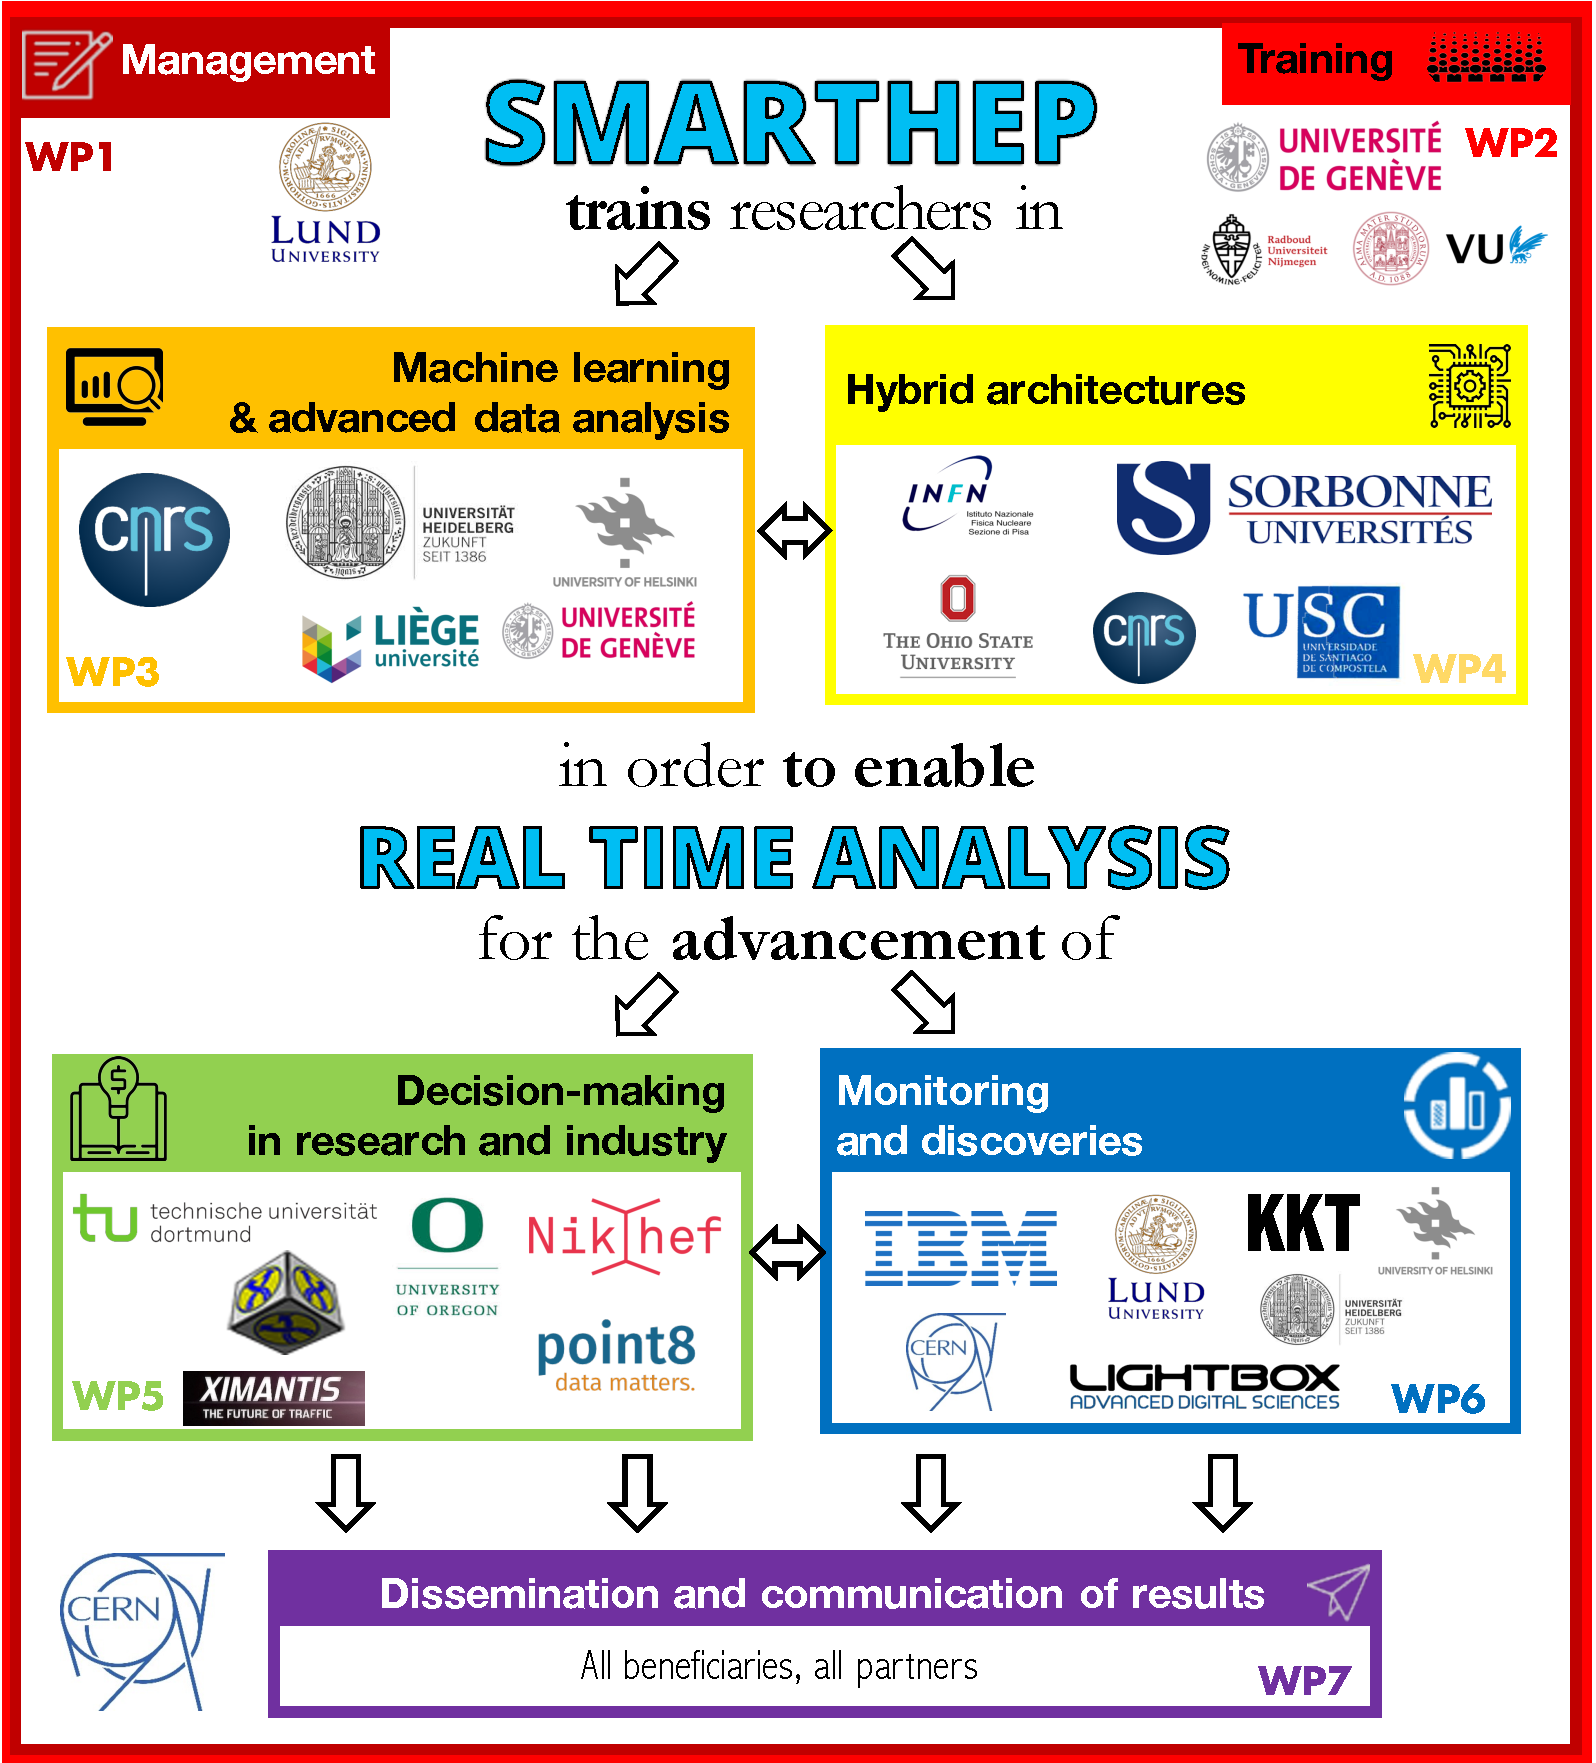
\includegraphics[width=0.6\textwidth]{figs/NetworkCompositionCombinedImplementation} %scienceStructure_2.pdf}
\begin{center}\footnotesize \label{fig:implementation}
Figure 1: \acronym implementation strategy and WPs. The nodes with their main expertise in a given WP are represented in the respective WP box.
\end{center}
\normalsize 
\vspace{-2mm}
\end{center}

%TODO: shorten this to one sentence, remove the blue
\subsubsection{Originality and innovative aspects of the research program} 
\label{sub:Originality}
%Expand on the state of the art: why is this original, innovative ad timely
%Refer to the state of the art in the first paragraph

The ESRs in the \acronym network will undertake a timely and ambitious research program on RTA, benefitting from the experience not only of their direct supervisors, but of the entire network, to reach their objectives. Some of the original and innovative aspects of the projects in the network are listed below. 

\noindent {\color{blue}{1. Researchers from \acronym process large datasets using RTA techniques in a cost-effective way}.}
A part of the novelty of this proposal is the volume of data which will be processed in real-time, comparable to the largest commercial tasks, but on a much smaller budget. 
%Instead of generating data that 
% MLD this is a great sentence but it is just out of place here
%This is true across both academic and non-academic applications:
%an estimated 90$\%$ of generated data is considered too expensive to store\footnote{\href{http://www.mckinsey.com/insights/business_technology/big_data_the_next_frontier_for_innovation}{2010 report on Big Data by McKinsey\&Company.}}.
One can compare Facebook and e.g. the LHCb collaboration.
%MLD I switched to numbers because then the comparison is more powerful (also shorter!)
The former 
%processes $O(100)$ petabytes of data per year and 
spends hundreds of millions of dollars a year on computing\footnote{Facebook, \href{http://www.datacenterknowledge.com/the-facebook-data-center-faq-page-three/}{The Facebook Data Center FAQ}, 2010.} while the latter only 
spends order 10M dollars a year on computing~\footnote{Private communication, \href{mailto:peter.clarke@ed.ac.uk}{Prof. Peter Clarke}, University of Edinburgh.}. 
% processes  $O(1000)$ petabytes of data per year and spends around 7M dollars a year on computing
%The essential difference is that Facebook stores and distributes this data to its users while LHC experiments largely process and then dispose of the data.
%MLD I felt this was not needed to make the above argument. It removes your figure 3 but see my comment from the email. 
%An example of this are the physics searches and measurements performed solely using trigger information.
%In these searches only a small fraction of each event, regardless of whether LHC experiments are able to record it for offline reconstruction or not, is saved for further processing. 
%This overcomes the storage limitations and allows to be more than an order of magnitude more sensitive to certain new particles (e.g. associated to Dark Matter, as in Fig.3).
To maintain a cost-effective data taking strategy, LHC experiments need a more systematic application of RTA (especially fully RTA-based analysis that discards bulky raw data), machine learning and hybrid architectures for HEP. 
As RTA is essential in industry as well as in HEP, the research environment can benefit from cross-pollination in terms of research topics, and from a generation of ESRs with experience in industrial grade algorithms and tools. 

\noindent {\color{blue}{2. The \acronym research program could lead to breakthroughs in our understanding of nature}}
Only fully-real time data acquisition techniques and trigger improvements enable full exploitation of the LHC dataset. 
The HEP research topics chosen to drive conceptual developments within \acronym have the potential to lead to the discovery of new physics beyond the Standard Model. 
%ESRs working on physics topics will target common challenges, e.g. when real-time algorithms and reconstruction techniques are not sufficiently advanced to distinguish signal from noise, or when the statistical power of the dataset is not fully exploited if objects are reconstructed with traditional techniques. 
Examples include studies of lepton flavor and its conservation and universality in different final states and experiments, dark matter mediators and new light particles, precise probes of the Higgs boson and of heavy ion physics, as well as not-yet-theorized phenomena that would not be possible to record using the current state-of-the-art triggers. 

\noindent {\color{blue}{3. ESRs in \acronym deploy and disseminate their research at a unique time for particle physics}.}
As highlighted by the HEP Software Foundation Whitepaper$^{4}$, the period 2019-2023 is ideal for this R\&D in HEP, as it is a time of transition between LHC data taking periods that will be necessary to prepare for an upgrade of the LHC accelerator where the amount of data delivered will make RTA techniques the key to pursue the physics programs of the four main LHC experiments.
The systematic optimization of HEP experiments by \acronym will boost the performance of the current and planned upgrades of the CERN based accelerator experiments.
Furthermore, the developed toolkits will be advertised at international conferences and thus the developed methods will shape the online event selection of all future HEP experiments. 
%The next LHC run (Run-3) will be starting in 2021 and the following one (Run-4) will begin in 2026.  
%Therefore, the 2020-2024 period is an ideal time for performing trigger upgrades and commissioning them with data, following the LHC upgrades that will deliver a much larger dataset than what is currently available. 

\noindent {\color{blue}{4. \acronym researchers further the RTA paradigm in both HEP and industry}.}
The close links of the research institutes of the consortium with the industry partners means that the ESRs will directly drive the development of novel industrial products, while also bringing professional methods of data mining that are exercised in large companies into the academic environment. 
Most modern methods applied in research can in this way be transferred to industry applications. 
By exposing industry-grade methods to the volume and complexity of HEP data, we will stimulate their development in a complementary way for the benefit of industry.
In particular, the ESRs will be trained in topics matching the emerging trend of real-time big data analytics\footnote{\href{https://www.scnsoft.com/blog/real-time-big-data-analytics-comprehensive-guide}{A comprehensive guide to real-time big data analytics.}} by invited speakers from large enterprises using these methods.   

% in automotive traffic optimization (ESR1-2, 6, 8) and analysis of sensor data for IoT and medical applications (ESR3-4, 9, 11, 13, 15).
%JA: not , 14 (??)) 
%The proposed algorithms and the use of ML methods on these scales of data are novel to both HEP and industry. 


